\chapter{User guide}

\section{Installation and use}
 
\subsection{Agents creation}

The Main program allows the user to control most of the simulation parameters.
From the spawning loop, the user chooses the number of agents involved for each type, the most important parameter for the simulation remaining the number of Attendants which deeply influences the performances :\\

\begin{figure}[h]
	\begin{minted}[bgcolor=bg,tabsize=4]{java}
for(int i = 0; i < 100; i++) {
	FrameworkLauncher.launchAgent(new Attendant(AttendantGender.MAN));
	FrameworkLauncher.launchAgent(new Attendant(AttendantGender.WOMAN));
}
	\end{minted}
\end{figure}

Apart from that, the user can decide to more specific agents as Stand Owners or Medics for a more realistic simulation, for example we usually spawn a seller for each stand as we limited their size in order not to overload the map with unnecessary occupied space.

\begin{figure}[h]
	\begin{minted}[bgcolor=bg,tabsize=4]{java}
for(Stand elem : standSet) {
	FrameworkLauncher.launchAgent(new Seller(elem));
}
	\end{minted}
\end{figure}

\subsection{Objects creation}

The class WorldModel is at work here. It basically simulates the whole environment in the program.
The method build() is where the code which creates and positions the objects on the map.
Subfonctions are called inside the function build for each object category that allows the user to place a number n of objects at the coordinates x,y and arrange them in a rectangle of height h and width w.

\newpage

\begin{figure}[h]
	\begin{center}
		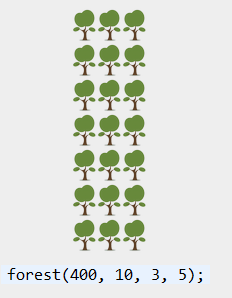
\includegraphics[width=0.3\textwidth]{img/forest.png}
	\end{center}
	\caption{Example of a forest}
\end{figure}

\section{GUI control documentation}
 
The GUI presents 2 controls, one to plant a bomb and one to exit the simulation. in order to plant a bomb in the festival, you just need to click somewhere on the map. A timer will then starts on the screen and people should start panicking if everything is done correctly.
